\begin{figure}[htbp]
  \centering
  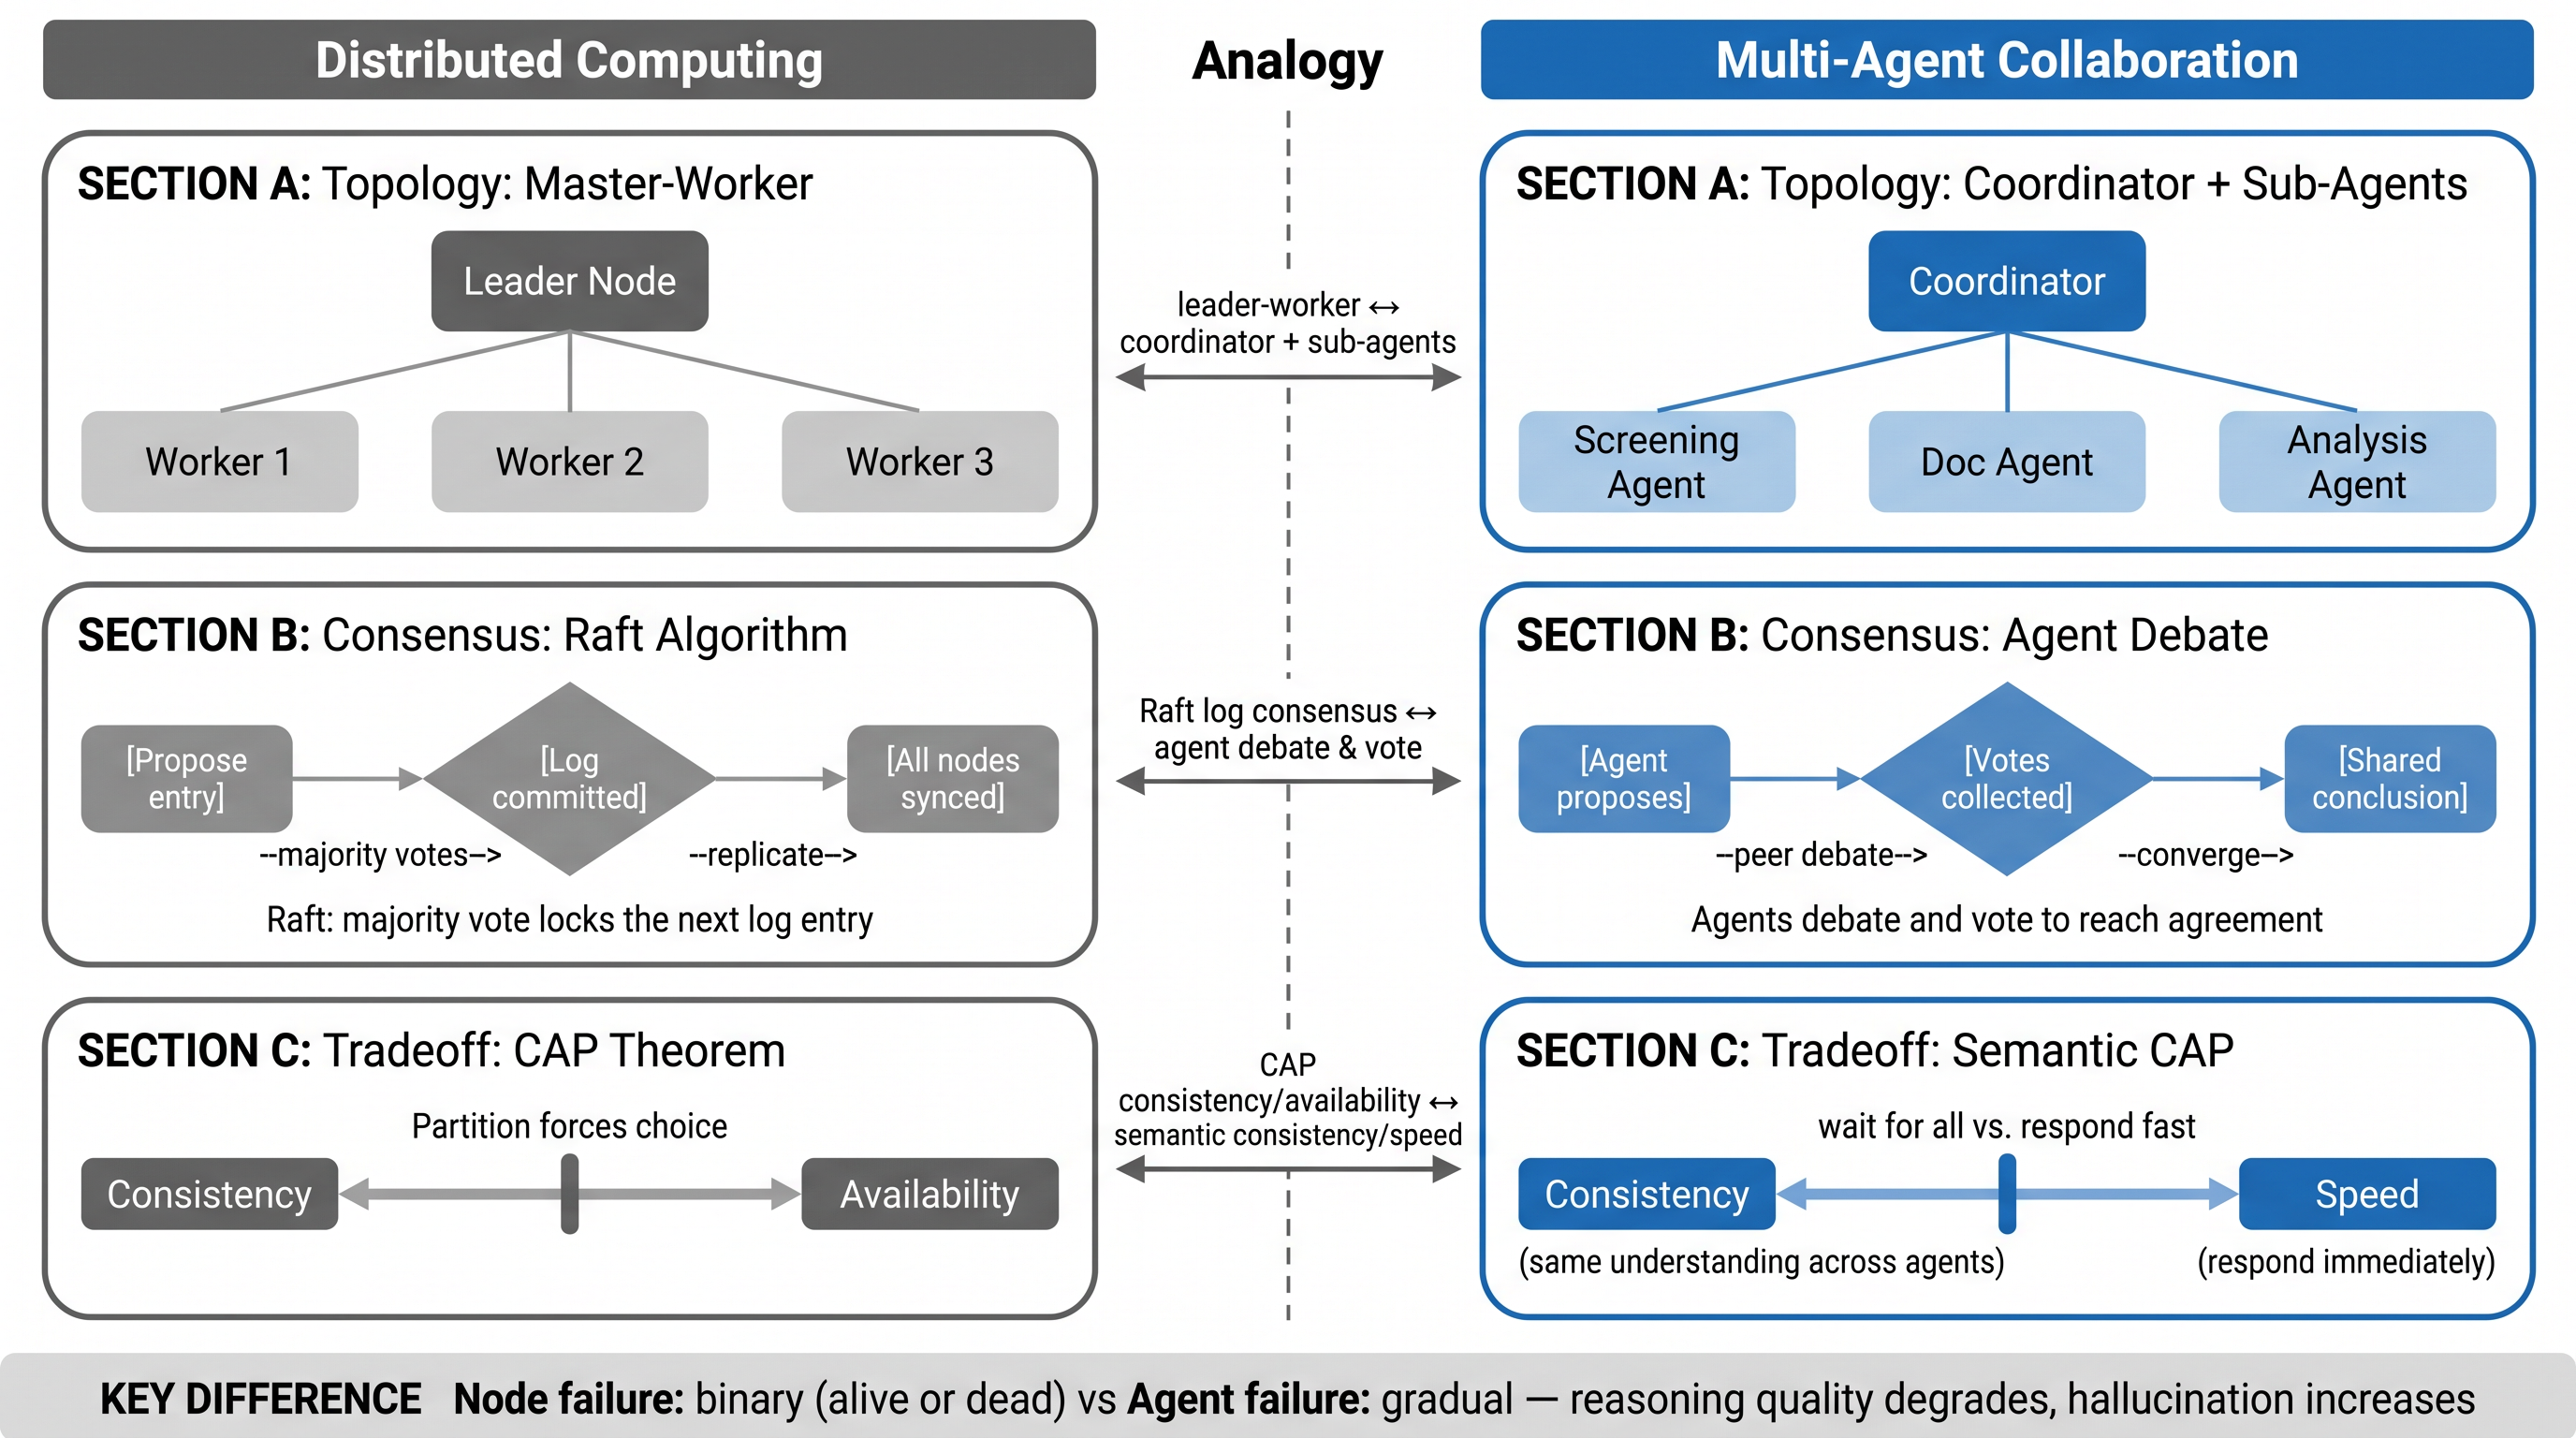
\includegraphics[width=0.9\textwidth]{figures/generated/fig_comp_56_multiagent}
  \caption{Multi-agent collaboration as distributed computing with semantics (§\ref{sec:distributed}).
  Both domains face the same coordination topologies (hub-and-spoke, pipeline, peer-to-peer)
  and the same fundamental tension between consistency and availability (CAP theorem /
  semantic CAP: wait for all agents vs.\ respond fast).
  The critical difference is failure mode: distributed-node failure is binary (alive or dead),
  whereas agent failure is gradual---reasoning quality degrades continuously through
  hallucination, task drift, and goal misalignment.}
  \label{fig:comp56:multiagent}
\end{figure}
